\documentclass[a4paper,12pt]{article} % тип документа

%  Русский язык
\usepackage{mathtext}               % русский язык в формулах
\usepackage[T2A]{fontenc}			% кодировка
\usepackage[utf8]{inputenc}			% кодировка исходного текста
\usepackage[english,russian]{babel}	% локализация и переносы

\usepackage{graphicx}               % импорт изображений
\usepackage{wrapfig}                % обтекаемые изображения
\graphicspath{{pictures/}}          % обращение к подкаталогу с изображениями
\usepackage{amsfonts}               % буквы с двойными штрихами
\usepackage{indentfirst}            % indent first
\usepackage{amsmath}                % можно выводить фигурные скобочки -- делать системы уравнений
\usepackage[table,xcdraw]{xcolor}   % таблицы
\usepackage{amsmath,amsfonts,amssymb,amsthm,mathtools} % Математика
\usepackage{wasysym}                % ???
\usepackage{upgreek}                % ???  

\usepackage{gensymb} % degree symbol
\usepackage{mathrsfs}

\usepackage{tikz}
\usetikzlibrary{graphs,graphs.standard}

\usepackage{cancel} % перечеркивания

%% Интервалы
\linespread{1}
\usepackage{multirow}

%% Перенос знаков в формулах (по Львовскому)
\newcommand*{\hm}[1]{#1\nobreak\discretionary{}
	{\hbox{$\mathsurround=0pt #1$}}{}}

%% Русские списки
\usepackage{enumitem}
\makeatletter
\AddEnumerateCounter{\asbuk}{\russian@alph}
\makeatother

% Дополнительная работа с математикой
\usepackage{amsmath,amsfonts,amssymb,amsthm,mathtools} % AMS
\usepackage{icomma} % "Умная" запятая: $0,2$ --- число, $0, 2$ --- перечисление

\usepackage{dsfont}
\usepackage{cancel} % перечеркивания

%%% Свои команды
\DeclareMathOperator{\sgn}{\mathop{sgn}}

%%% Программирование
\usepackage{etoolbox} % логические операторы

\usepackage{marvosym}
\usepackage{wasysym}

%%% Страница
\usepackage{extsizes} % Возможность сделать 14-й шрифт
\usepackage{geometry} % Простой способ задавать поля
	\geometry{top=20mm}
	\geometry{bottom=20mm}
	\geometry{left=20mm}
	\geometry{right=20mm}
	
\usepackage{mathrsfs}

\newcommand{\eqdef}{\stackrel{\mathrm{def}}{=}}
\newcommand{\ryad}{\sum\limits^{\infty}_{k = 0}}

\newcommand{\R}{\mathbb{R}}
\newcommand{\N}{\mathbb{N}}
\newcommand{\series}{\sum\limits_{k=1}^{\infty}}
\newcommand{\useries}{\sum\limits_{k=1}^{\infty} u_k}
\newcommand{\useriesl}{\sum\limits_{k=1}^{\infty} u_k < \infty}
\newcommand{\useriese}{\sum\limits_{k=1}^{\infty} u_k = \infty}
\newcommand{\auseries}{\sum\limits_{k=1}^{\infty} |u_k|}
\newcommand{\auseriesl}{\sum\limits_{k=1}^{\infty} |u_k| < \infty}
\newcommand{\auseriese}{\sum\limits_{k=1}^{\infty} |u_k| = \infty}
\newcommand{\sn}{\sum\limits_{k=1}^{n} u_k}

\renewcommand {\ge}{\geqslant}
\renewcommand {\le}{\leqslant}
\renewcommand {\geq}{\geqslant}
\renewcommand {\leq}{\leqslant}
\renewcommand {\epsilon}{\varepsilon}

\usepackage{titlesec}
\titlelabel{\thetitle.\quad}
%%% Для точек после названий секций

\usepackage{hyperref}
%%% Настройка ссылок
\hypersetup
{
	colorlinks = true,
	linkcolor  = black,
	filecolor  = magenta,
	urlcolor   = blue
}
%%% Конец настройки ссылок


\begin{document}

%=======================================================================================

\begin{titlepage}
\begin{center}
\
\vfill

{\LARGE \textsc{\textbf{Программное моделирование прохождения непараксиальных лучей через тонкую линзу\\}}}

\vspace{2em}

Фатыхов Тимур\\ Гончаренко Валентина\\2 курс ФРКТ, группа Б01-009

\vfill

Май 2022
\end{center}
\end{titlepage}

%=======================================================================================

\newpage
\tableofcontents{} %содержание
\newpage

%1
%=======================================================================================

\section{Введение}

Предыстория вопроса по выбору весьма витиеватая - так как мы студенты физтех-школы компьютерных технологий, то хотели оправдать это название и совместить физику с посильными нам задачами на компьютере. Изначально мы планировали написать модель дискретных полярных сияний на Марсе, чтобы можно было пронаблюдать их точечное возникновение наглядно в зависимости от различных параметров, которые могли задаваться <<by hand>>. Нам пришлось отказаться от этой идеи, так как при детальном рассмотрении физика явления оказалась не слишком <<оптична>>, несмотря на иллюзорно кажущееся прямое отношение к визуальным феноменам. К тому же, необходимо было учитывать ограничения по нашей компетентности в сфере програмирования, что существенно сужало круг рассматриваемых вариантов проекта. Несколько раз модифицируя курс наших усилий, мы пришли к воплощению прохождения непараксиальных лучей через тонкую линзу.

\newpage

\section{Условие поставленной задачи с точки зрения физики}
Необходимо найти формулу, связывающую положение предмета и изображения, даваемого тонкой собирающей линзой, в случае, когда угол между лучом и оптической осью нельзя считать малым. На основе полученной формулы качественно проанализировать изменения изображения по сравнению с изображением, построенным по правилу, справедливому для параксиальных лучей.

\section{Решение поставленной задачи и вывод формулы}
Изображение какого-либо объекта можно построить по точкам, поэтому достаточно вывести формулу, связывающую положение точечного источника и его изображения.

Рассмотрим предварительно вспомогательную задачу. Вычислим угол отклонения луча, проходящего через треугольную призму, относительно его первоначального направления. Будем считать угол $\alpha$ при вершине призмы малым, что соответствует приближению тонкой линзы.

\textbf{Формулировка вспомогательной задачи:} на кварцевый клин с углом при вершине $\alpha$ падает из воздуха луч света под углом $\beta$ к нормали к поверхности клина. Под каким углом $\gamma$ к нормали к другой поверхности луч выходит из клина в воздух? Коэффициент преломления кварца $n$.

\textbf{Решение:} Возможны три случая хода луча. Рассмотрим случай произвольных углов $\alpha$ и $\beta$. Возможный ход лучей в призме показан на рис.1 (а, б, в).

\begin{figure}[h!]
	\centering
	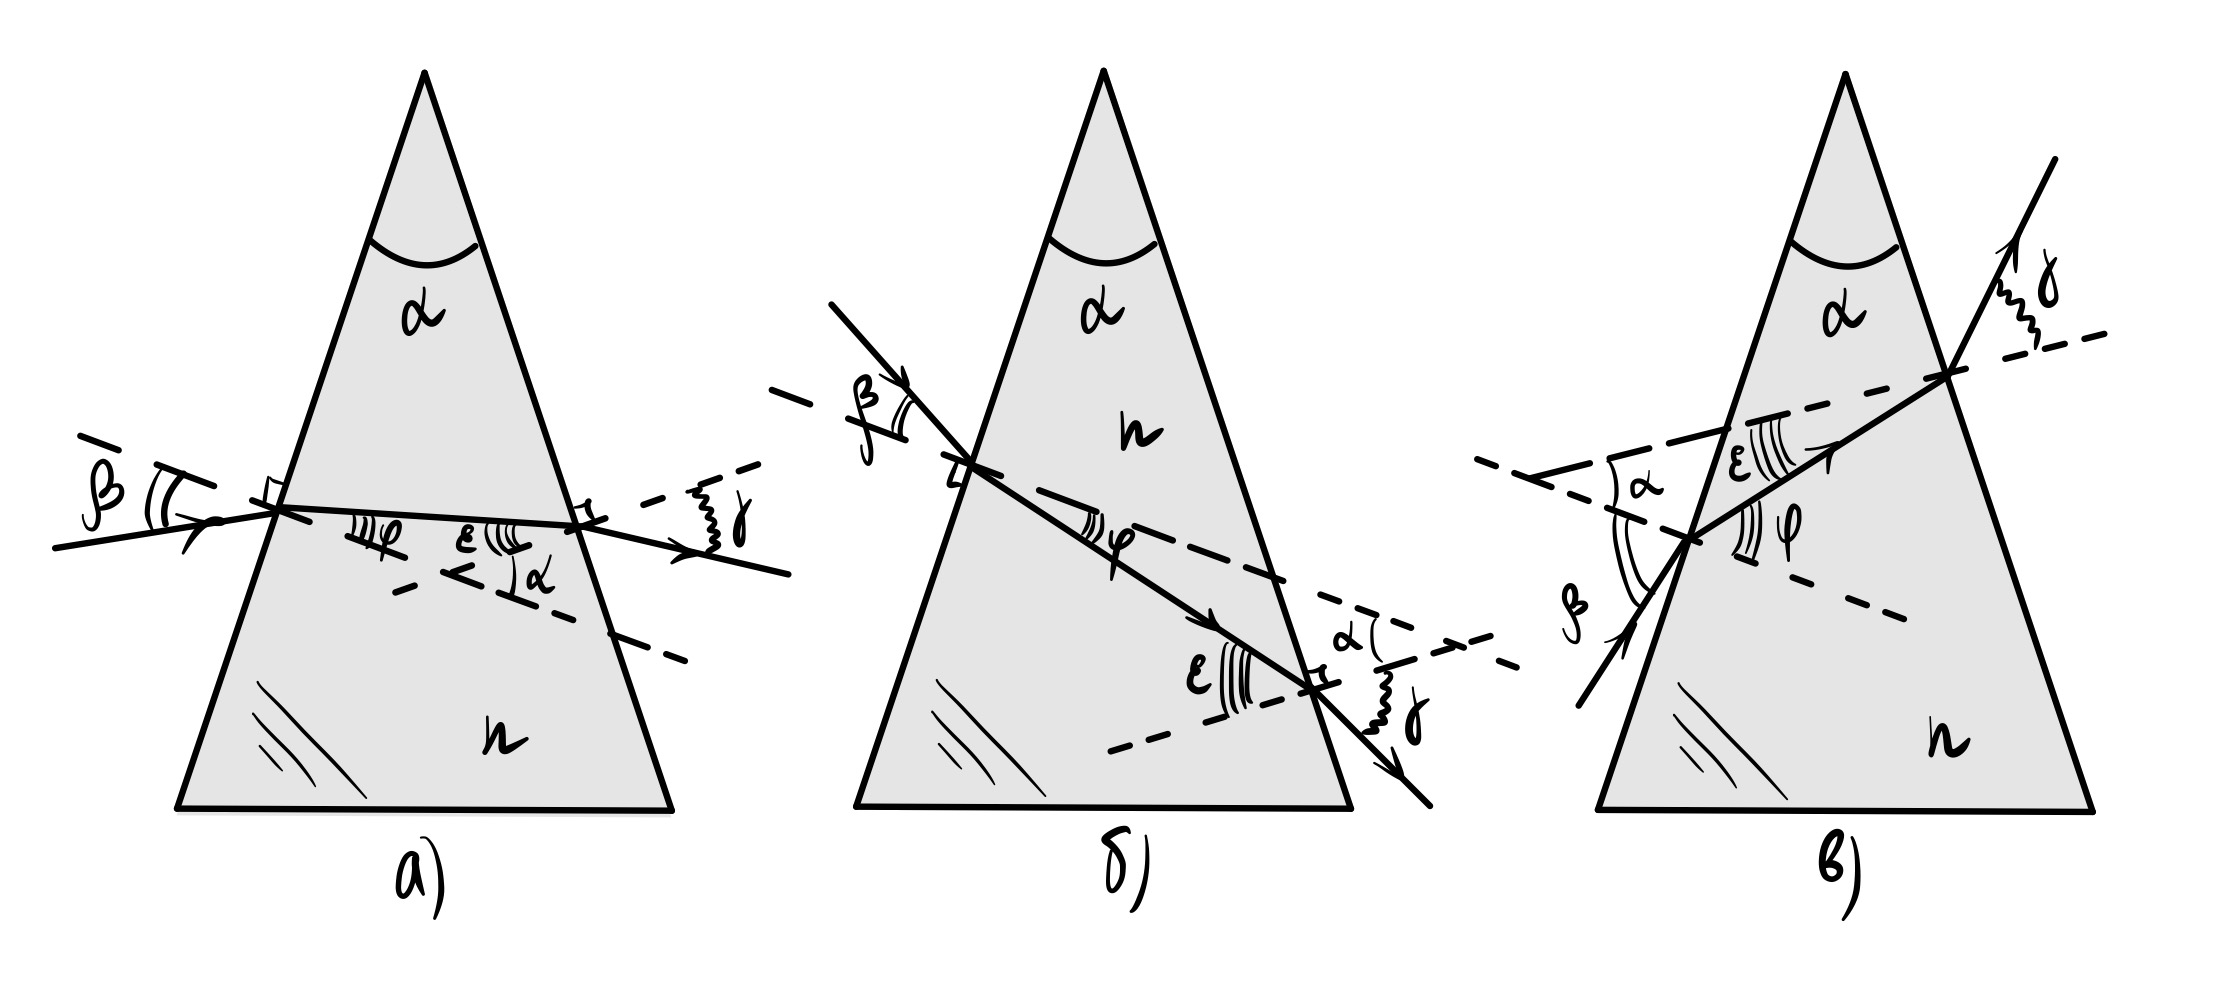
\includegraphics[scale=0.22]{IMG_1466.JPG}
	\caption{Три случая хода луча}
\end{figure}

Во всех случаях выполняется закон преломления на обеих боковых поверхностях клина:
$$
\frac{\sin \beta}{\sin \varphi}=n ; \quad \frac{\sin \gamma}{\sin \varepsilon}=n .
$$
На рис. 1(а) $\varepsilon=\alpha-\varphi$. Поэтому
$$
\begin{aligned}
&\sin \gamma=n \sin \varepsilon=n \sin (\alpha-\varphi)=n(\sin \alpha \cos \varphi-\cos \alpha \sin \varphi)= \\
&=n\left(\sin \alpha \sqrt{\frac{n^{2}- \sin ^{2} \beta}{n^{2}}}-\cos \alpha \frac{\sin \beta}{n}\right)=\sin \alpha \sqrt{n^{2}-\sin ^{2} \beta}-\cos \alpha \sin \beta .
\end{aligned}
$$
На рис. 1(б) $ \varepsilon=\alpha+\varphi$. Имеем:

$\sin \gamma=n \sin \varepsilon=n \sin (\alpha+\varphi)=n(\sin \alpha \cos \varphi+\cos \alpha \sin \varphi)=$
$$
=n\left(\sin \alpha \sqrt{\frac{n^{2}-\sin ^{2} \beta}{n^{2}}}+\cos \alpha \frac{\sin \beta}{n}\right)=\sin \alpha \sqrt{n^{2}-\sin ^{2} \beta}+\cos \alpha \sin \beta.$$
На рис. 1 (в) $ \varepsilon=\varphi-\alpha$. В этом случае
$$
\begin{aligned}
&\sin \gamma=n \sin \varepsilon=n \sin (\varphi-\alpha)=n(\sin \varphi \cos \alpha-\cos \varphi \sin \alpha)= \\
&=n\left(\frac{\sin \beta}{n} \cos \alpha-\sqrt{\frac{n^{2}-\sin ^{2} \beta}{n^{2}}} \sin \alpha\right)=\sin \beta \cos \alpha-\sin \alpha \sqrt{n^{2}-\sin ^{2} \beta} .
\end{aligned}
$$

Воспользуемся рисунками и обозначениями, приведенными в задаче выше. Для первого разобранного в решении случая угол отклонения от первоначального направления луча $\delta$ связан с углами, приведенными на рисунке, соотношением $\delta=\beta-\varphi+\gamma-\varepsilon$.

Во втором случае формула, приведенная в решении, и формула для $\delta$ получаются из формул первого случая заменой $\beta, \varphi$ на $-\beta,-\varphi$. Соответственно, решение и формула для $\delta$ в третьем случае получается заменой $\gamma, \varepsilon$ на $-\gamma,-\varepsilon$. Таким образом, достаточно рассмотреть только первый случай, для которого
$$
\sin \gamma=\sin \alpha \sqrt{n^{2}-\sin ^{2} \beta}-\cos \alpha \sin \beta .
$$
Учтем далее малость угла $\alpha$ и пренебрежем слагаемыми порядка $\alpha^{2}$ и выше. Мы получим соотношение $\sin \gamma+\sin \beta = \alpha \sqrt{n^{2}-\sin ^{2} \beta}$. Преобразуем это выражение к виду
$$
2 \sin \left(\frac{\gamma+\beta}{2}\right) \cos \left(\frac{\gamma-\beta}{2}\right)=\alpha \sqrt{n^{2}-\sin ^{2} \beta} .
$$
Правая часть этого выражения стремится к нулю при $\alpha \rightarrow 0$. Поскольку углы $\gamma$ и $\beta$ меньше $\pi / 2$, это возможно лишь при малом значении $\gamma+\beta$. Так как при этом $\beta \approx-\gamma$, значение косинуса в последнем выражении можно с той точностью, с которой производятся вычисления, заменить на $\cos \beta$. В результате получим соотношение
$$
(\gamma+\beta) \cos \beta=\alpha \sqrt{n^{2}-\sin ^{2} \beta} .
$$
Учитывая, что $\alpha=\varepsilon+\varphi$, получим для угла $\delta$ выражение
$$
\delta=\beta-\varphi+\gamma-\varepsilon = \beta + \gamma - \alpha
$$
$$
\delta=\alpha\left(\frac{\sqrt{n^{2}-\sin ^{2} \beta}}{\cos \beta}-1\right) .
$$
Заметим, что это выражение справедливо для всех трех случаев, рассмотренных выше.

Применим это выражение для нахождения координат изображения точечного источника. Выберем систему координат так, как указано на рис. 2. Пусть точечный источник находится в точке $A$ с координатами $\left(x_{1}, y_{1}\right)$, а его изображение - в некоторой точке $B$, координаты которой $\left(x_{2}, y_{2}\right)$ необходимо найти. Для нахождения положения изображения воспользуемся двумя лучами. Первый луч проходит через центр линзы без преломления. Уравнение соответствующей лучу прямой имеет вид: $y=k x$, где $k=y_{1} / x_{1}$. Второй луч пустим под небольшим углом $\psi$ по отношению к первому.

\begin{figure}[h!]
	\centering
	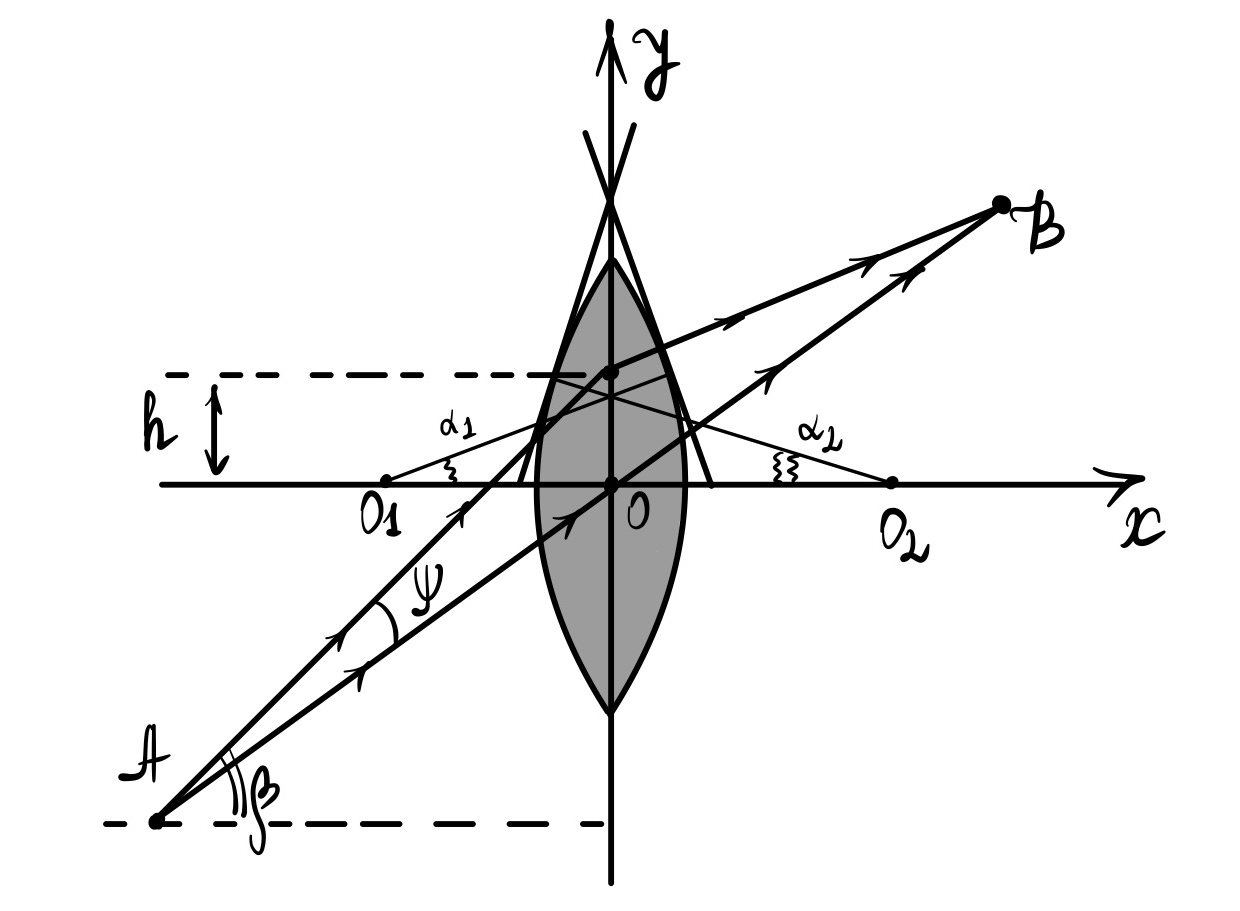
\includegraphics[scale=0.32]{IMG_1467.JPG}
	\caption{К нахождению координат изображения}
\end{figure}

Проходя через линзу, этот луч поворачивается на некоторый угол. Чтобы определить угол поворота, заменим линзу призмой, грани которой касаются линзы в точках, где этот луч пересекает поверхность линзы.

Чтобы определить угол при вершине призмы, проведем из центров сфер поверхностей линзы (точки $O_{1}$ и $O_{2}$) отрезки к точкам касания. Углы между отрезками и оптической осью обозначим через $\alpha_{1}$ и $\alpha_{2}$. Эти отрезки ортогональны поверхностям линзы и, соответственно, поверхностям построенной призмы. Основываясь на геометрических соображениях, можно доказать, что угол при вершине призмы $\alpha$ связан с этими углами соотношением: $\alpha=\alpha_{1}+\alpha_{2}$. Этот угол входит в ранее выведенное выражение для $\delta$ и определяет ход второго луча после прохождения линзы. Пересечение этого луча с первым лучом дает точку $B$.

Второй (рассмотренный только что) луч проходит линзу (и соответствующую призму) на расстоянии $h$ от оптической оси. В приближении тонкой линзы можно считать, что три точки - пересечение лучом первой поверхности линзы, пересечение лучом второй поверхности и пересечение лучом плоскости линзы одинаково удалены от оптической оси. Величина $h$ связана с углом $\psi$ соотношением
$$
\operatorname{tg}(\beta+\psi)=\frac{\left|y_{1}\right|+h}{\left|x_{1}\right|} .
$$
Выражая $y_{1}$ через $x_{1}$, получаем соотношение
$$
h=\frac{\left|x_{1}\right| \operatorname{tg} \psi}{(1-\operatorname{tg} \beta \operatorname{tg} \psi) \cos ^{2} \beta} .
$$
Будем рассматривать лучи, проходящие через линзу вблизи ее оптического центра. Поэтому, считая угол $\psi$ малым, приходим к соотношению, справедливому для любых $\beta<\pi / 2$ :
$$
h=\frac{\left|x_{1}\right|}{\cos ^{2} \beta} \psi .
$$
C другой стороны, величину $h$ можно связать с радиусами кривизны линзы: $h=R_{1} \sin \alpha_{1} \approx R_{1} \alpha_{1} \approx R_{2} \alpha_{2}$. Замена синусов углов углами соответствует приближению тонкой линзы. Используя это выражение и выражение для $h$, угол $\alpha$ можно выразить через угол $\psi$ :
$$
\alpha=h\left(\frac{1}{R_{1}}+\frac{1}{R_{2}}\right)=\frac{\left|x_{1}\right|}{\cos ^{2} \beta}\left(\frac{1}{R_{1}}+\frac{1}{R_{2}}\right) \psi=\frac{\left|x_{1}\right|}{\cos ^{2} \beta} \frac{n-1}{f} \psi .
$$
В этом выражении величина $f-$ фокусное расстояние тонкой линзы, определяемое для параксиальных лучей:
$$
\frac{1}{f}=(n-1)\left(\frac{1}{R_{1}}+\frac{1}{R_{2}}\right) .
$$
Уравнение, определяющее прямую, по которой идет второй луч после прохождения линзы, имеет вид $y=k^{\prime} x+h$. Величина $k^{\prime}$ определяется через соответствующий угол:
$$
k^{\prime}=\operatorname{tg}(\beta-\psi+\delta) \approx \operatorname{tg} \beta+\frac{\delta-\psi}{\cos ^{2} \beta}=k+\frac{\delta-\psi}{\cos ^{2} \beta} .
$$
Поскольку точка $B$ находится на пересечении двух лучей, ее координаты определяются в результате решения системы уравнений:
$$
\begin{aligned}
&y_{2}=k x_{2}, \\
&y_{2}=k^{\prime} x_{2}+h,
\end{aligned}
$$
что с учетом равенства для $k'$ приводит к уравнению для $x_{2}$ :
$$
\frac{\delta-\psi}{\cos ^{2} \beta} x_{2}+h=0 .
$$
Используя выведенные ранее соотношения, выразим угол $\delta$ через угол $\psi$, величину $h$ также выразим через угол $\psi$. В результате после подстановок и некоторых преобразований получим уравнение относительно $x_{2}$ :
$$
\left(\frac{\left|x_{1}\right|}{\cos ^{2} \beta} \frac{n-1}{f}\left(\frac{\sqrt{n^{2}-\sin ^{2} \beta}}{\cos \beta}-1\right)-1\right) x_{2}=\left|x_{1}\right| .
$$
Учтем теперь, что $\left|x_{1}\right|=-x_{1}$, и выразим синус и косинус угла $\beta$ через тангенс, т. е. через $k$. В результате соотношение, определяющее значение $x_{2}$, можно привести к виду
$$
\frac{1}{x_{2}}-\frac{1}{x_{1}}=\frac{1}{f}\left(1+k^{2}\right) \frac{\sqrt{n^{2}+\left(n^{2}-1\right) k^{2}}-1}{n-1} .
$$
Величина $y_{2}$ связана с величинами $x_{2}, x_{1}$ и $y_{1}$ указанным выше соотношением в системе уравнений, подставляем и находим явно. Полученные формулы определяют связь между координатами точечного источника и его изображения в случае, когда луч, идущий от источника через линзу, не является параксиальным. 


Проведем анализ полученных выражений. Для параксиального луча угол $\beta$ и, соответственно, величина $k$ малы. При $k \rightarrow 0$ выражение выше совпадает с обычно используемой формулой для тонкой линзы (с учетом знака $x_{1}$). C возрастанием угла между падающим на линзу лучом и оптической осью возрастают поправки. Одно из качественных отличий заключается в том, что, если одну линзу заменить другой с тем же фокусным расстоянием, но другим показателем преломления (соответственно с другими радиусами кривизны), то изображение того же точечного источника сместится. Заметим, что, поскольку диапазон изменения показателя преломления незначителен, то, как показывают расчеты, этот эффект практически не проявляется.

Следствием изменения формулы, связывающей положение источника и изображения, является то, что для непараксиальных лучей геометрические правила построения изображений в тонкой линзе оказываются неприменимыми и все построения возможны лишь путем численного расчета. Некоторые качественные отличия получающихся изображений несложно понять, не прибегая к численному расчету. Так, например, при параксиальных лучах изображением отрезка прямой также является отрезок прямой. Это свойство можно вывести, исходя из правил геометрического построения изображений.

Если координаты точек объекта связаны линейным соотношением $y_{1 i}=a_{1} x_{1 i}+b_{1}$, то соответствующая линейная связь будет справедлива и для точек изображения: $y_{2 i}=a_{2} x_{2 i}+b_{2}$, где $a_{2}=a_{1}+b_{1}, b_{2}=b_{1}$. При отличном от нуля значении $k$ такая линейная связь пропадает, и изображением отрезка прямой становится кривая линия.

\begin{figure}[h!]
	\centering
	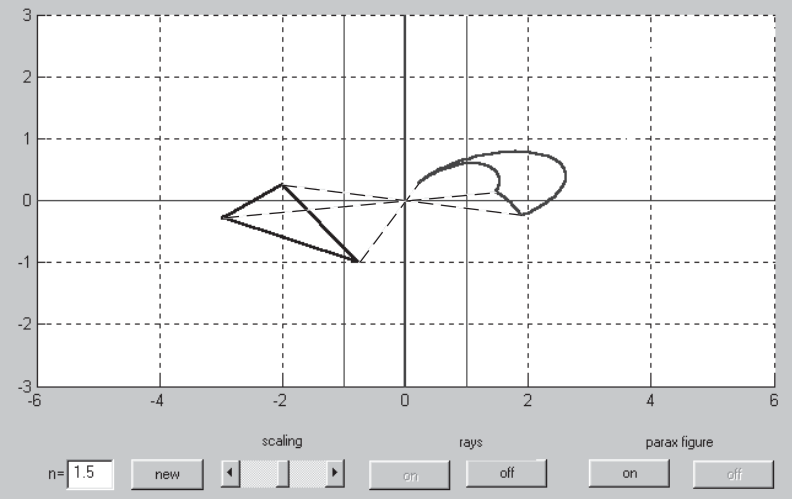
\includegraphics[scale=1.2]{png.png}
	\caption{Пример численного построения изображения}
\end{figure}

Пример построения изображения при численном расчете по выведенным формулам приведен на рисунке 3. Сплошная горизонтальная прямая на рисунке соответствует оптической оси, a сплошные вертикальные прямые - плоскости линзы и двум фокальным плоскостям $(f=1)$. Как видно из рисунка, лишь один из отрезков треугольника, для которого лучи можно считать параксиальными, дает изображение в виде отрезка. Из приведенного примера можно заметить еще одно свойство: если бы мы построили изображение приведенного треугольника по правилам, справедливым для параксиальных лучей, мы получили бы разорванную фигуру, так как два из отрезков треугольника пересекают фокальную плоскость. Однако в данном случае получается связная фигура.

Следствием вышесказанного является тот факт, что пучки параллельных лучей, идущие под большим углом к оптической оси, фокусируются уже не в фокальной плоскости. Точка фокусировки определяется выведенными формулами, в которых следует устремить $x_{1} \rightarrow-\infty$ (настройка на бесконечность). Вместо двух фокальных плоскостей образуются две фокальные поверхности с координатами $\left(x_{f}, y_{f}\right)$. Эти поверхности заданы параметрически уравнениями
$$
x_{f}=\frac{f(n-1)}{\left(1+k^{2}\right)\left(\sqrt{n^{2}+\left(n^{2}-1\right) k^{2}}-1\right)}, \quad y_{f}=k x_{f} .
$$

\begin{figure}[h!]
	\centering
	\includegraphics[scale=1.2]{дщд.png}
	\caption{Две фокальные поверхности}
\end{figure}

Из рис. 4 видно, насколько эти поверхности отличаются от плоскостей (расчет выполнен для $f=1, n=1,5, k \in[-1,1])$.
\newpage
\section{Основные этапы сборки с точки зрения программирования}
Программа написана на языке С++. Нам нужно было работать с графикой для отрисовки макета лупы, загрузки картинок, работы с пикселями и их координатами. Также нам нужно было создать объекты со свойствами точек предмета и изображения, создать саму линзу и функции конвертации точек предмета в точки изображения по формулам, которые справедливы для параксиальным лучей и непараксиальных лучей, чтобы пронаблюдать разницу. Код лежит в репозитории на сервисе <<GitHub>>, и при желании его можно посмотреть полностью. Для разделения труда и работы отдельно с графикой и физикой преобразования точек каждый писал свою часть работы, после этого мы объединили полученные куски программы. Было принято решение оставить увеличивающееся изображение полупрозрачным, чтобы эффект увеличения можно было сравнить с первоначальной картинкой. На рис.5 представлены воплощенные в коде функции конвертации точек предмета в точки изображения для параксиального и непараксиального случаев.

\begin{figure}[h!]
	\centering
	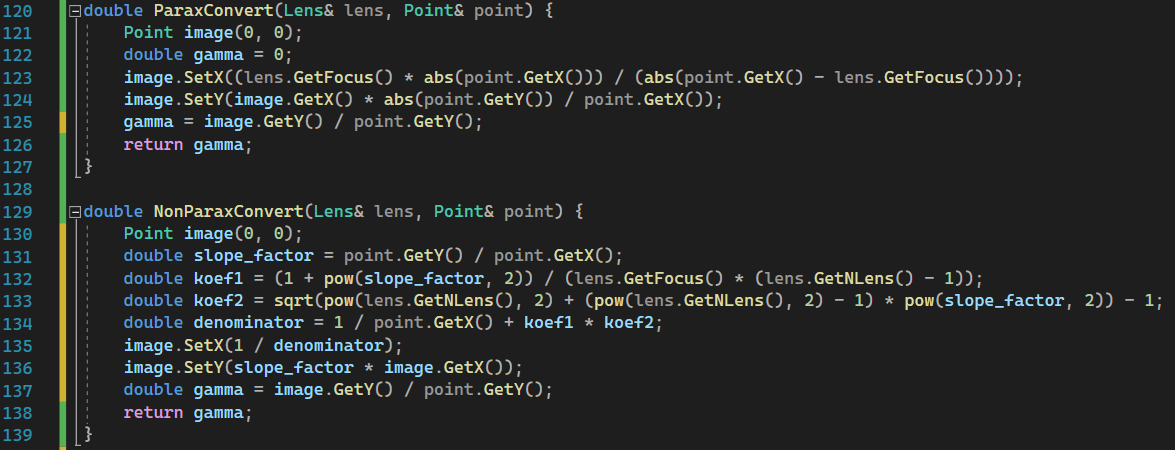
\includegraphics[scale=0.8]{image_2022-05-30_15-53-46.png}
	\caption{Функции для параксиальных и непараксиальных лучей}
\end{figure}

\newpage
\section{Результат}
Репозиторий с кодом можно найти по ссылке:

\url{https://github.com/vasyavasilevs/Non-approximated-ray-simulation/blob/valya/non_parax_rays_sim.cpp}

Ниже представлен результат работы программы для нескольких картинок. Также можно провести демонстрацию в онлайн-режиме.

\begin{figure}[ht]\center
\begin{tabular}{cc}
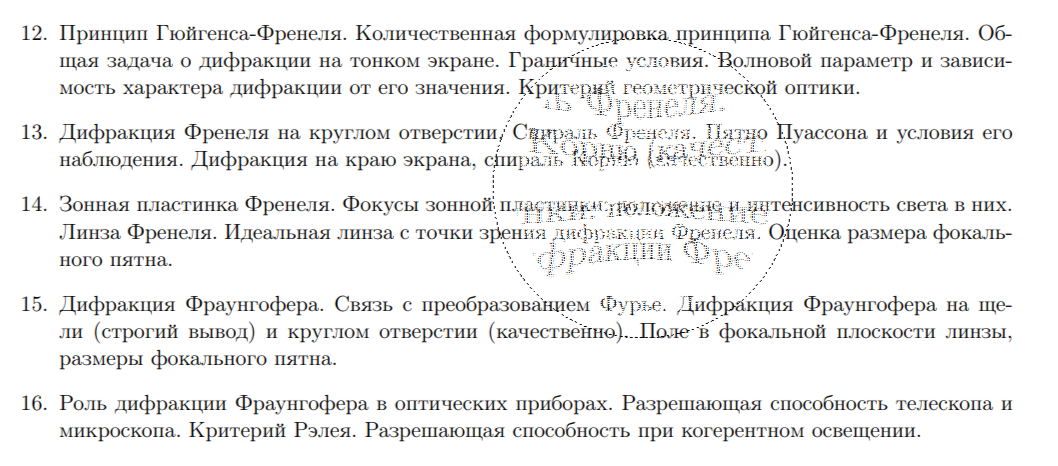
\includegraphics[width=85mm]{экз_нон.png}
&
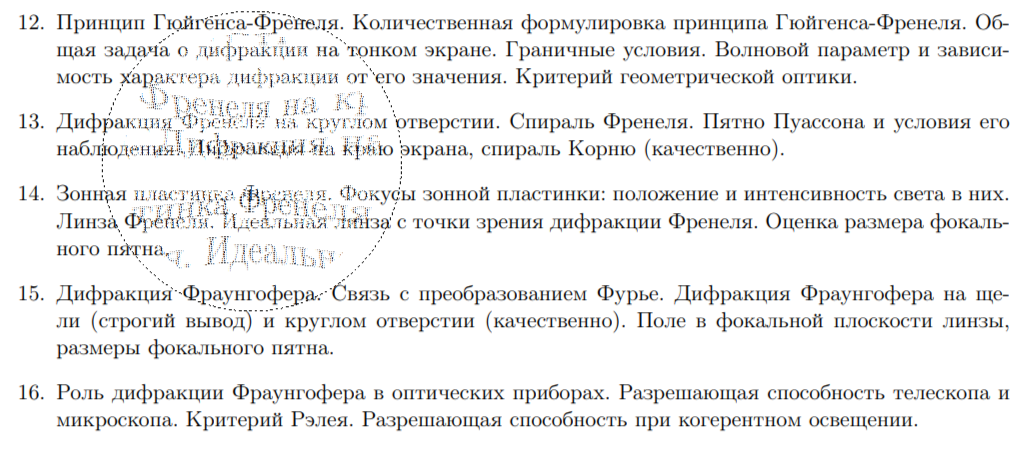
\includegraphics[width=85mm]{экз_нон2.png}
\end{tabular}
\caption{Непараксиальные лучи}
\end{figure}

\begin{figure}[h!]
	\centering
	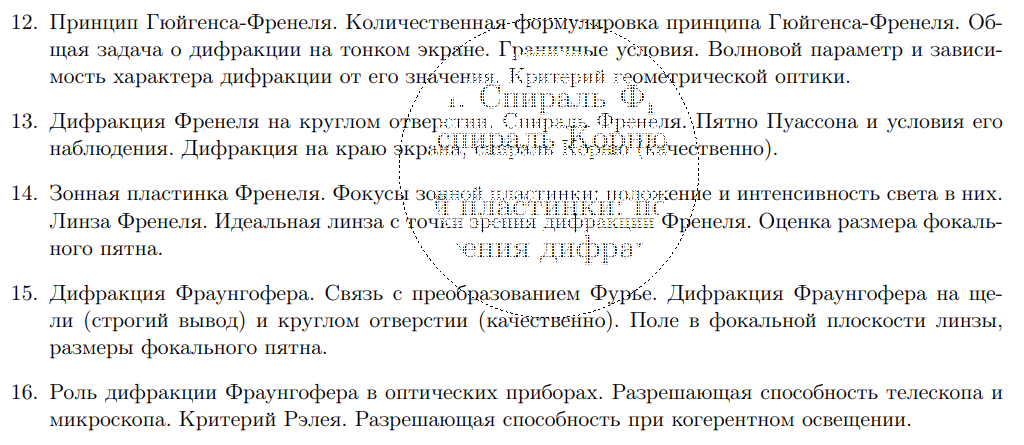
\includegraphics[scale=0.75]{экз_пара.png}
	\caption{Параксиальные лучи}
\end{figure}

\begin{figure}[ht]\center
\begin{tabular}{cc}

\includegraphics[scale=0.4]{тукс_нон.png}
&

\includegraphics[scale=0.4]{тукс_паракс.png}
\end{tabular}
\caption{Слева - непараксиальные лучи, справа - параксиальные}
\end{figure}

\begin{figure}[ht]\center
\begin{tabular}{cc}
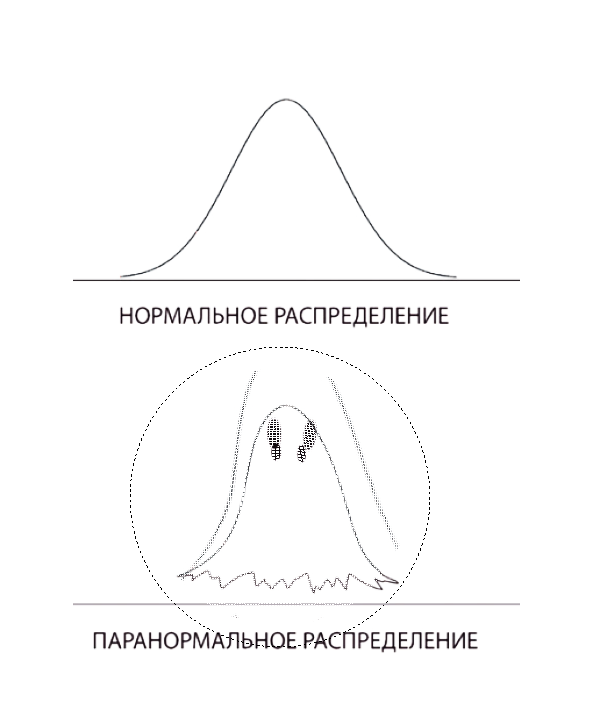
\includegraphics[width=80mm]{пара_нон1.png}
&
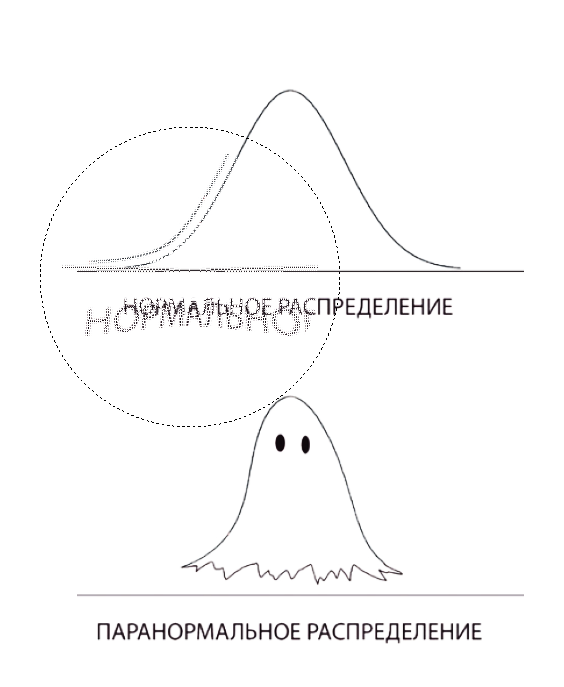
\includegraphics[width=80mm]{пара_нон2.png}
\end{tabular}
\caption{Непараксиальные лучи}
\end{figure}

\begin{figure}[h!]
	\centering
	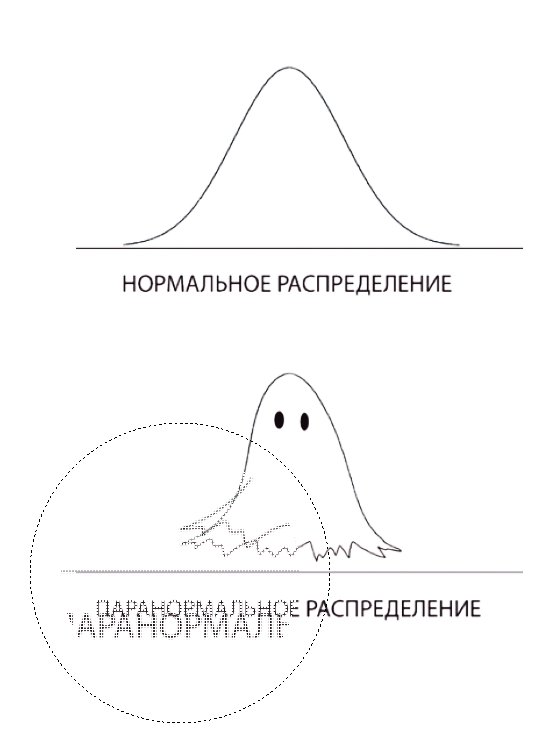
\includegraphics[scale=0.95]{пара_пара.png}
	\caption{Параксиальные лучи}
\end{figure}

\newpage

\section{Источники и ресурсы}

\begin{enumerate}
  \item Кондратьев А.С., Ляпцев А.В. Физика. Задачи на компьютере. ФИЗМАТЛИТ, 2008. 314-320 сс.

  \item Д.В. Сивухин, "Общий курс физики". Учеб. пособие: Для вузов. В 5 т. Т.IV. Оптика.
  
  \item Кондратьев А. С., Уздин В. М. Физика. Сборник задач. — М: Физматлит, 2005. — 392 с.

  \item Семинарские презентации и советы преподавателя по программированию (Миряха Владислав Андреевич).
  
  \item https://www.youtube.com/hashtag/simplecode
\end{enumerate}

\end{document}